%% psoc_api

API til styring af PSoC, herunder sensor og sprinkler, er implementeret i PSoC Creator. Top designet består af en ADC\_SAR\_Seq, en analog pin og to digitale pins til at styre henholdsvis sprinkler og Select til bestemmelse af temperatur- eller fugtighedsdata for SHT21P.
I top designet er der angivet følgende pins. ''ADC\_in'', ''SLC'', ''water\_pin'' disse forbindes til henholdsvis pin P2[5], P0[0] og P2[0]. ADC\_in oprettes som en analog pin og de to andre som digitale output pins. Under konfiguration for de digitale pins fravælges ''HW Connection'' under Digital Output. For nærmere opsætning af pins henvises til figur \ref{lab:water_pin_konfig} og figur \ref{lab:SLC_pin_konfig}

\begin{figure}[htb]
\centering
{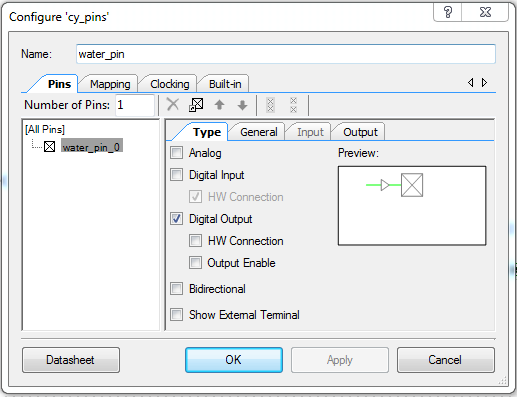
\includegraphics[width=0.70\textwidth]{filer/pics/water_pin_konfig.png}}
\caption{Konfig. for water pin}
\label{lab:water_pin_konfig}
\end{figure}


\begin{figure}[htb]
\centering
{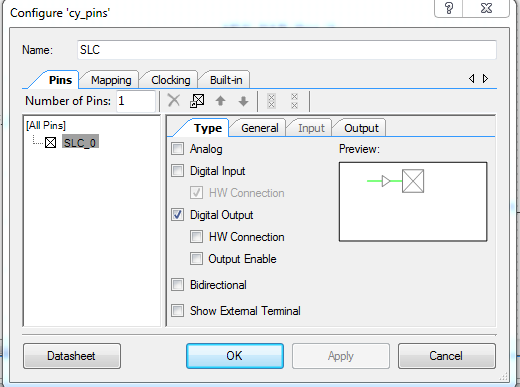
\includegraphics[width=0.70\textwidth]{filer/pics/SLC_pin_konfig.png}}
\caption{Konfig. for SLC pin}
\label{lab:SLC_pin_konfig}
\end{figure}  

Under konfiguration for ADC-komponenten vælges Vref til VDDA og Single ended negative input vælges til Vss. Dette sætter ADCen op til at bruge 0 V som reference spænding.

Da PSoC kun har en SAR komponent er det nødvendigt at initialisere denne i sensorPackage-driveren.

\begin{figure}[htb]
\centering
{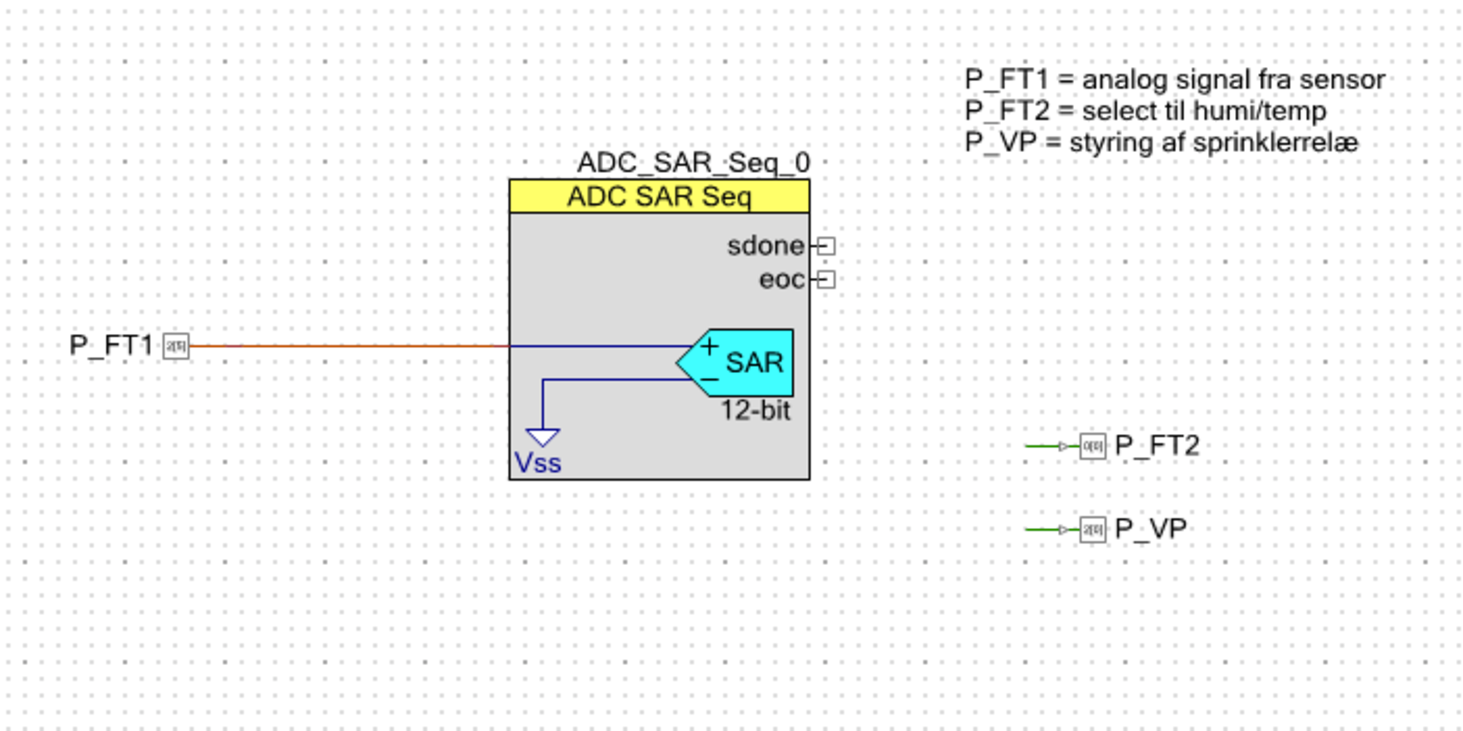
\includegraphics[width=0.70\textwidth]{filer/pics/psoc_api_topdesign.png}}
\caption{Top Design for PSoC API}
\label{lab:psoc_api_topdesign}
\end{figure}

\begin{figure}[htb]
\centering
{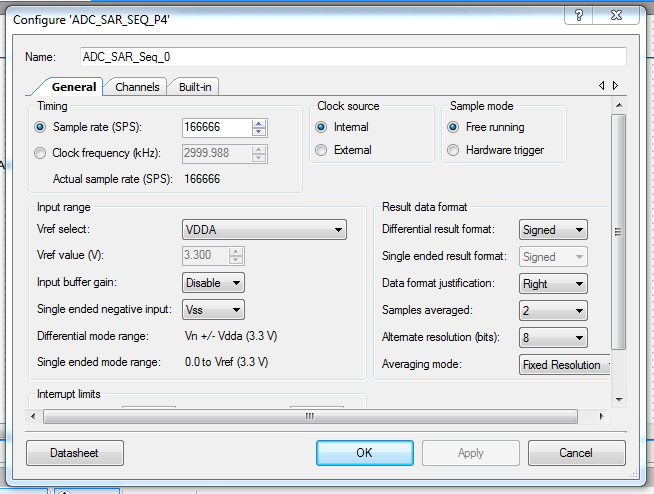
\includegraphics[width=0.70\textwidth]{filer/pics/psoc_api_config1.png}}
\caption{Konfiguration af Vref og Single ended negative input}
\label{lab:psoc_api_config1}
\end{figure}

\begin{figure}[htb]
\centering
{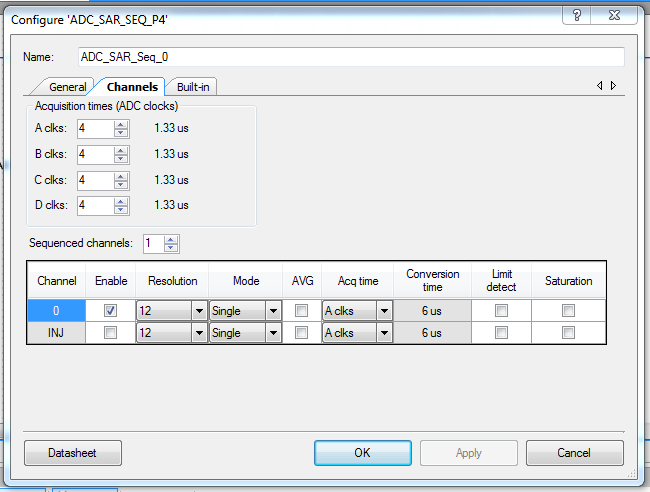
\includegraphics[width=0.70\textwidth]{filer/pics/psoc_api_config2.png}}
\caption{Konfiguration af Channels for PSoC API}
\label{lab:psoc_api_config2}
\end{figure}